\justifying
\begin{problem}{1}
	%(физика обл) 3%
	В одне з колін $U$ - подібної трубки з водою влили гас, після чого різниця рівнів в трубці дорівнювала $3$ см. У друге коліно доливали бензин доти, поки рівні рідини в обох трубках не стали рівними. Визначіть висоту стовпчика безину
\end{problem}

\begin{problem}{2}
	%физика обл 7%
	З дна озера намагаються підняти  затонулий сталевий якір масою $780$ кг за допомогою пінопластової кулі, яку прикріплюють до якоря легким тросом. При якому мінімальному об'ємі кулі це мождиво? Густини сталі, води та піномласту відповідно дорівнюють $7800,~1000, ~750 \dfrac{\text{кг}}{\text{м}}^3$
\end{problem}



\begin{problem}{4}
	%18%
	Тіло плаває на поверхні ртуті так, що в неї занурено $0.25$ його об'єму. Яка частина тіла буде занурена в ртуть, якщо зверх неї налити шар води, який повністю покриває тіло?
\end{problem}

\begin{problem}{5}
	%22%
	В $U$ - подібну трубку з площами колін $S_1$ та $S_2$ налили воду. Як зміниться рівень води в $U$ - подібній трубці, якщо в одне коліно кинули кусок дерева масою $m$, а в інше коліно -- кусок пінопласту такої ж маси?
\end{problem}

\begin{problem}{6}
	%28%
	
	Два циліндри з'єднані внизу трубкою. В один з них налили води, а в інший -- нафти. При цьому різниця нафти і води буда $h = 5$ см. Переріз циліндра з нафтою дорівнював $S = 80~\text{см}^2$. У циліндр з нафтою поклали невагоммий поршень і деякий вантаж на поршень. При якій масі вантажу рівні води і нафти будуть однакові? 
\end{problem}

\begin{problem}{7}
	%33%
	
	В $U$ - подібну трубку постійного перерізу налили води. Після цього в ліве коліно налили рідини з меншою густиною по вінця трубки (до краю). В праве коліно кинули кусок деревини масою $m$ визначіть об'єм рідини, яка виллється.
\end{problem}







\begin{problem}{14}
	%8.5 2014 All-ukr%
	
	Струмінь води, що витікає з крана, звужується донизу. Знайти залежність діаметра $d$ струменя води від відстані $l$ до крана. Початкова швидкість витікання води $v_0$, діаметр отвору крана $d_0$.
\end{problem}

\begin{problem}{15}
	%15.73  ZNO%
	
	На горизонтальній поверхні стола стоїть широка посудина з водою. Висота води в посудині дорівнює $h$, маса посудини з водою -- $M$. У бічній поверхній посудини є отвір, площа якого $S$, закритий корком. ПРи якому коефіцієнті тертя між дном та столом посудина почне рухатись, якщо вийняти корок?
\end{problem}

\textbf{Задачі для самостійного розв'язання}

\begin{problem}{3}
	%физика обл 14%
	У рідині з постійною швидкістю повільно опускається кулька радіуса $R$ та маси $m$. Яку масу мала б кулька того ж радіуса, щоб вона піднімалась з тією ж швидкістю, з якою опускається перша кулька? Густини рідини $\rho$, сила опору пропорційна швидкості
\end{problem}

\begin{problem}{8}
	%64%
	
	Для того, щоб при плаванні у гліцерині об'єм зануреної частини дерев'яного бруска дорівнював об'єму зануреної частини при плаванні його у воді. на брусок додатково наантажили $13$ Н. Визначіть вагу бруска. (густина гліцерину -- $1.26~\dfrac{\text{г}}{\text{см}^3}$)
\end{problem}

\begin{problem}{9}
	%ЗНО приклад 2%
	
	Рівень води в $U$ - подібній трубці розміщений на $30$ см нижче від її верхніх країв. Ліву трубку повністю заповнюють гасом, густина якого $800~\dfrac{\text{кг}}{\text{м}^3}$. Визначте висоту стовпа гасу в трубці.
\end{problem}

\begin{problem}{10}
	Шматок металу, маса якого дорівнює $1$ кг, при повному зануренні у воду важить $8$ H, а при повному зануренні у невідому речовину важить $8.4$ Н. Визначте густину невідомої рідини.
\end{problem}

\begin{problem}{11}
	Повітряна куля наповнена воднем. Маса оболонки й обладнання дорівнює $300$ кг. Скільки людей може підняти куля, якщо середня маса однієї людини дорівнює $70$ кг? Густина повітря $1.29~\dfrac{\text{кг}}{\text{м}^3}$
\end{problem}

\begin{problem}{12}
	Однорідну кулю підвісили на пружині. Після занурення системи в мастило, густиною $900 ~\dfrac{\text{кг}}{\text{м}^3}$, видовження пружини зменшилося в 3 рази. Визначте ггустину матеріау кулі.
\end{problem}

\begin{problem}{13}
	%15.71 ZNO%
	Вода тече зі швидкістю $2 ~\dfrac{\text{м}}{\text{с}}$ по горизонтальній трубі, площа поперечного перерізу якої $2 ~\text{м}^2$. Труба плавно звужується  до перерізу $1 ~\text{м}^2$. На скільки зміниться статичний тиск води?
\end{problem}

\begin{problem}{14}
	%197 Kozlov%
	
	У два коліна $U$ - подібної трубки налито вода та мастило, які розділені ртуттю (див. рис. \ref{fig:koz197}). Поверхні розділу ртуті і рідини в обох рідинах знаходяться на однаковій висоті. Знайти висоту стовпа води $h_0$, якщо висота стовпа мастила $h = 20$ см. Густина мастила $\rho = 0.9\cdot 10^3 ~\dfrac{\text{кг}}{\text{м}^3}$, води $\rho = 1\cdot 10^3 ~\dfrac{\text{кг}}{\text{м}^3} $
	
	\begin{figure}[h!]
		\centering
		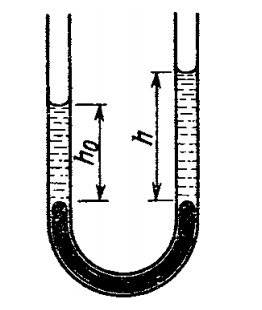
\includegraphics[width=0.2\linewidth]{class9/koz_197}
		\caption{}
		\label{fig:koz197}
	\end{figure}
	
\end{problem}